%----------------------------------------------------------------------------
% Unofficial LaTex beamer theme for Seoul National University
%
% 
%----------------------------------------------------------------------------

\documentclass[compress]{beamer}
\usepackage{beamerthemeshadow}
\usetheme{snubeam}
\usepackage{snucode}

\begin{document}
\title{예시 Beamer 타입의 \LaTeX 문서}
\author{Sungwoo Park}
\institute{
    Uncertainty Quantification Lab\\
    Seoul National University}
\date{August 19, 2025}

{
% \usebackgroundtemplate{\includegraphics[width=\paperwidth]{images/snu-shift}}
\begin{frame}[plain]
  \titlepage
\end{frame}
}

\begin{frame}\frametitle{Table of contents}
    \tableofcontents
\end{frame}

\section{Introduction}
\begin{frame}\frametitle{Beamer 작성 시 유의할 점}
	\begin{itemize}
		\item Beamer는 프레젠테이션을 위한 LaTeX 클래스입니다.
		\item \href{https://github.com/snudm/snubeam}{SNU Beamer} 테마를 사용한 템플릿입니다.
		\item 도큐먼트와 다르게, 해당 파일도 같이 있어야 합니다.
		\begin{itemize}
            \item beamerthemesnubeam.sty
            \item snucode.sty
            \item ref.bib
        \end{itemize}
        \item 각 파일의 쓸모는 알아서 잘 찾아보세요...
	\end{itemize}
\end{frame}

\begin{frame}\frametitle{Brief Introductions about TabPFN}
	\begin{itemize}
		\item TabPFN: A Transformer that solves small tabular classification problems in a second \cite{Hollmann2022-op}
		\item \alert{TabPFNv2}: Accurate predictions on small data with a tabular foundation model \cite{Hollmann2025-pr}
		\item Fast tabular statistical model using transformer.
		\item The distribution of the prediction is calculated in this formula.
		\begin{align*}
			p(y | x, D) = \int_{\Phi} p(y|x,\phi)p(D|\phi)p(\phi)d\phi
		\end{align*}
	\end{itemize}
\end{frame}

\begin{frame}\frametitle{Structure of TabPFN}
	\begin{enumerate}
		\item Pre-training
		\begin{itemize}
			\item Model is trained on synthetic datasets (created by SCM) by
			minimizing the discrepancy between the predicted label of the
			test instance and its true label
			\item We don't know the pre-training phase's structure : In the pip library, it just downloads pre-trained parameters and performs the inference phase.
		\end{itemize}
		\item Inference
		\begin{itemize}
			\item For given data (training set + test set), TabPFN performs \alert{a single forward pass} to generate predictions for all test samples.
			\item In inference phase, model only do in-context learning, not backpropagation
		\end{itemize}
	\end{enumerate}
\end{frame}

\begin{frame}[fragile]\frametitle{TabPFN Example}
	Here is an example for fitting and making a prediction using TabPFN:
	\begin{pythoncode}
		>>> from tabpfn import TabPFNRegressor
		>>> ....
		>>> train_1 = pd.DataFrame(data = [[-2, -2], [-1, -1], [1, 1], [2, 2]],
		columns = ['x', 'y'])
		>>> test = pd.DataFrame(data = [[0]], columns = ['x'])
		>>> regressor = TabPFNRegressor(device = 'cuda')
		>>> regressor.fit(train_1[['x']], train_1[['y']]) // Forward pass
		>>> regressor.predict(test) // Prediction
		    array([0.1495245], dtype=float32)
	\end{pythoncode}
	\begin{tabular}{|c|}
		\hline
		\textbf{x} \\ \hline
		-2 \\ \hline
		-1 \\ \hline
		1 \\ \hline
		2 \\ \hline
	\end{tabular}, 
	\begin{tabular}{|c|}
	\hline
	\textbf{y} \\ \hline
	-2 \\ \hline
	-1 \\ \hline
	1 \\ \hline
	2 \\ \hline
	\end{tabular} $\xrightarrow{\text{TabPFNRegressor}}$ regressor, \begin{tabular}{|c|}
	\hline
	\textbf{x}  \\ \hline
	0  \\ \hline
	\end{tabular}  $\xrightarrow{\text{regressor}}$ \begin{tabular}{|c|}
	\hline
	\textbf{y}  \\ \hline
	2 \\ \hline
	\end{tabular}
	
\end{frame}

\section{Performance}
\begin{frame}\frametitle{Is TabPFN better then traditional statistical models?}
	\begin{itemize}
		\item In the past, many studies show that traditional statistical models (XGBoost, Random Forest, etc.) still outperform most deep learning models on tabular data. \cite{Shwartz-Ziv2021-mo}, \cite{Grinsztajn2022-fl}
		\item But TabPFN claims that their model is a state-of-the-art model for tabular data.
	\end{itemize}
\end{frame}

\begin{frame}\frametitle{Why does this happen?}
	\begin{itemize}
		\item TabPFN excels in handling small- to medium-sized  datasets with up to 10,000 samples and 500 features. For larger datasets and highly non-smooth regression  datasets, approaches such as CatBoost, XGB or AutoGluon are likely to outperform TabPFN. \cite{Hollmann2025-pr}
		\item The model was trained on a synthetic dataset generated via an SCM with about 130 million dataset samples.
		\item Since the dataset covered only a limited value range, the model did not learn to generalize beyond that domain.
	\end{itemize}
\end{frame}

\subsection{Time Series}

\begin{frame}\frametitle{TabPFN-TS}
	\begin{itemize}
		\item Hoo et al., 2025 proposed TabPFN-TS, a TabPFN variant specific for time series.
		\item Proposes optimal transformation (preprocess) strategies tailored for TabPFN with time series data.
	\end{itemize}
\end{frame}

\begin{frame}\frametitle{TabPFN-TS: Preprocessing}
	\begin{itemize}
		\item Running index: chronological order
		\item Calendar features: second, minute, hour, weekday, day (month), day (year), week (year), year
		\item Seasonal features:
		\begin{itemize}
			\item Additional cycles (e.g., lunar, non-calendar periodicities)
			\item FFT top-$k$ frequency features ($k=5$)
		\end{itemize}
		\item Cyclic features: sin / cos transformation
		\[\Phi(t) = \left(\cdots, \cos \left(\frac{2 \pi t}{P_i}\right), \sin \left(\frac{2 \pi t}{P_{i}}\right), \cdots\right)\]
	\end{itemize}
\end{frame}

\begin{frame}\frametitle{TabPFN-TS vs XGBoost}
	\begin{itemize}
		\item In the paper, there is no comparison with XGBoost
		\item We conducted experiments using the Chronos \cite{ansari2024chronos} m4\_hourly 100 time series datasets, predicting the last 48 data points.
		\item For a fair comparison, XGBoost was trained with the same feature set as TabPFN-TS.
	\end{itemize}
\end{frame}

\begin{frame}\frametitle{TabPFN-TS vs XGBoost}
	\begin{itemize}
        \item hi
		\begin{columns}
			\begin{column}{5cm}
				\begin{figure}
					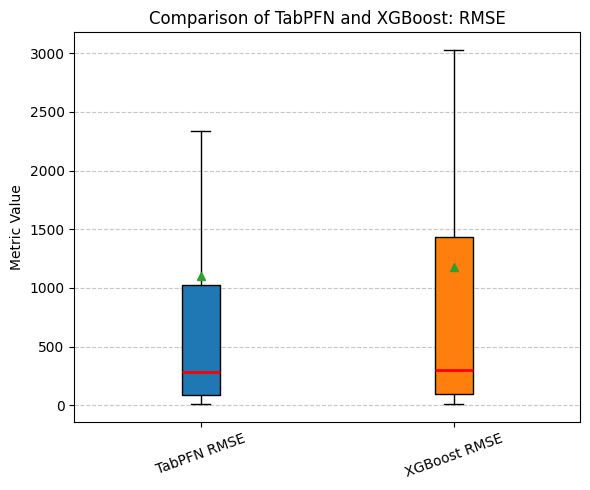
\includegraphics[width = 5cm]{images/fig_ts_rmse.png}
				\end{figure}
			\end{column}
			\begin{column}{5cm}
				\begin{figure}
					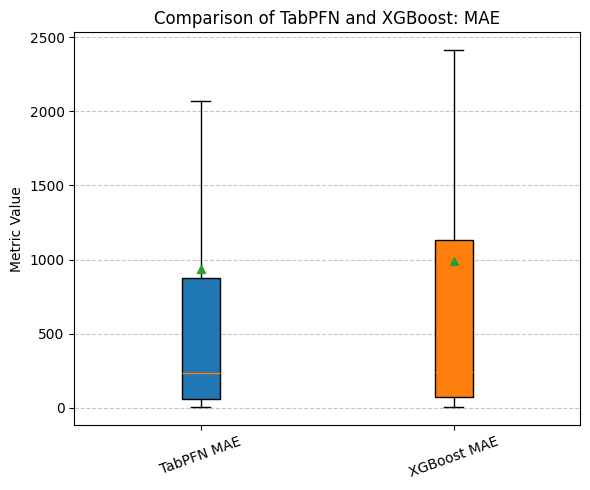
\includegraphics[width = 5cm]{images/fig_ts_mae.png}
				\end{figure}
			\end{column}			
		\end{columns}
        \item hello
	\end{itemize}
\end{frame}


\begin{frame}\frametitle{TabPFNv2 vs others}
	\begin{itemize}
		\item Hello
	\end{itemize}
	\begin{figure}
		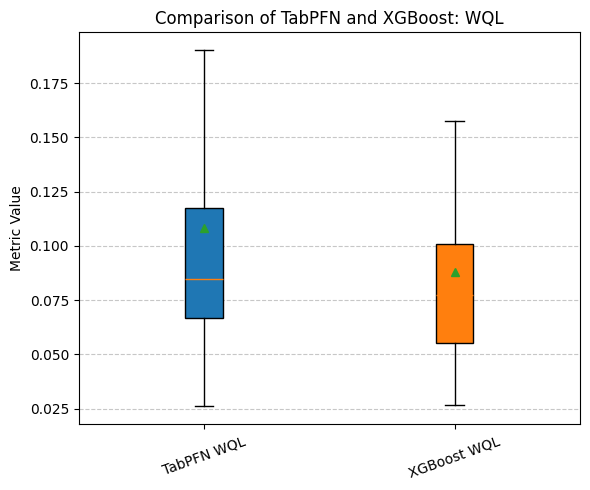
\includegraphics[width = 5cm]{images/fig_ts_wql.png}
	\end{figure}
\end{frame}

\section{Conclusion}
\begin{frame}\frametitle{Conclusion}
	\begin{itemize}
		\item 안녕
	\end{itemize}
\end{frame}

\begin{frame}\frametitle{}
    \vfill
    \begin{center}
        \begin{Huge}Thank you!\end{Huge}
    \end{center}
    \vfill
\end{frame}

\begin{frame}[t, allowframebreaks]\frametitle{References}
    \nocite{*} % FIXME: this includes all references in ref.bib
    \bibliography{ref}
\end{frame}
\end{document}
